\chapter{INSTALASI QGIS}

Cara instalasi aplikasi QGIS berbeda antara menggunakan sistem operasi Windows dan sistem operasi Linux.

\begin{enumerate}[A.]

\item Instalasi QGIS di lingkungan Sistem Operasi Windows

Untuk sistem operasi Windows, perangkat lunak QGIS dapat di unduh secara gratis di \textit{website} resmi QuantumGIS dengan alamat http://qgis.org/ melalui berbagai macam \textit{web browser} seperti Firefox, Chrome, Opera, atau Internet Explorer. Tahapannya adalah sebagai berikut :

\begin{enumerate}[1.]

\item Pada kolom halaman di atas jendela \textit{browser}, masukan teks berikut dan tekan Enter : http://qgis.org/, sehingga muncul jendela pada gambar \ref{fig:qgishomepage} :

\begin{figure}
  \centering
  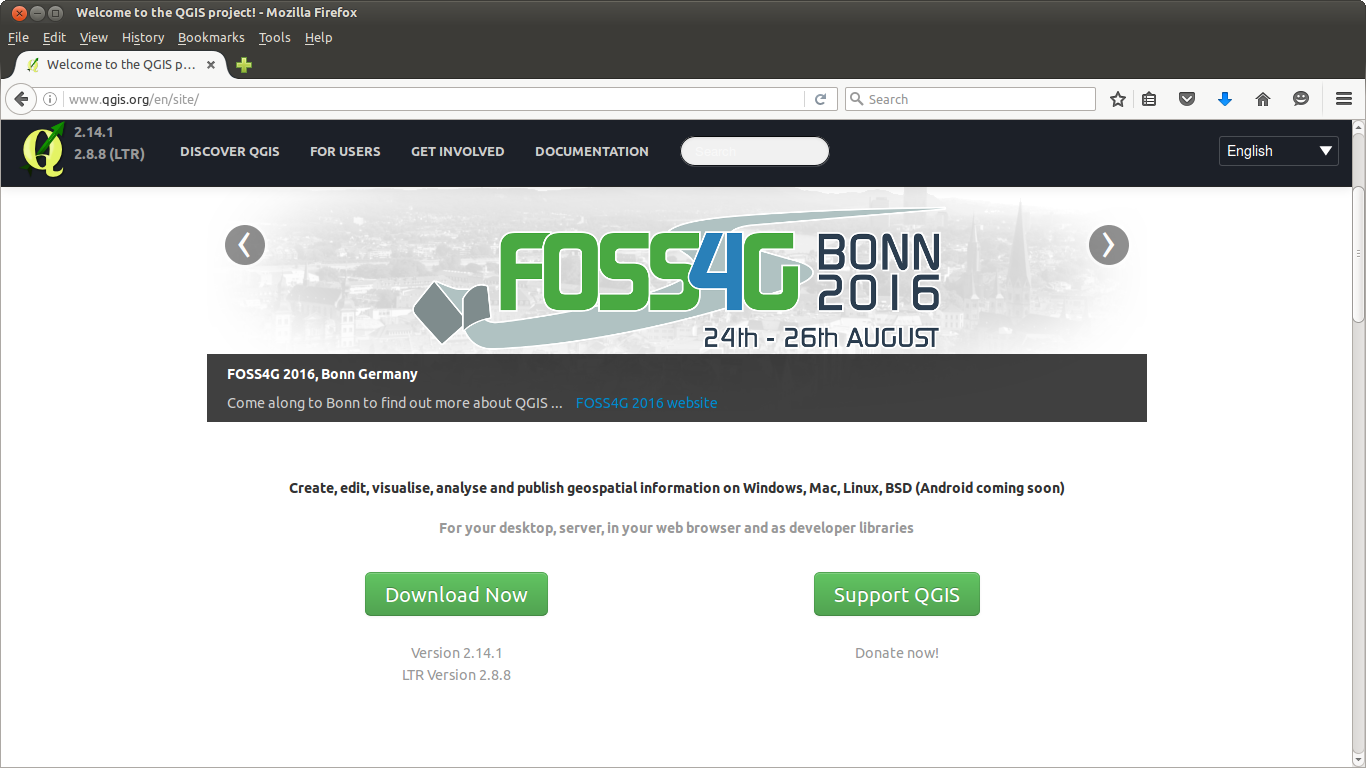
\includegraphics[width=1\textwidth]{./resources/001-homepage-qgis}
  \caption{Jendela \textit{website} QGIS}
  \label{fig:qgishomepage}
\end{figure}

\item Klik \verb|Download Now| pada halaman tersebut.

\end{enumerate}

\item Instalasi QGIS di lingkungan Sistem Operasi Linux (Debian/Ubuntu)

\end{enumerate}